
\subsection{Approximating an Optimal Path}\label{sec:LP}
In this section an approach to finding a global optimal solution to the optimisation problem proposed in Section \ref{sec:optiprob}. The optimisation problem is a non-linear optimisation problem, due to \( D(e_i)/v_{e_i} \) and $R_{CO}(v_{e_i})$ being non-linear functions. The problem can however be reformulated into a linear programming problem by reformulating \( D(e_i)/v_{e_i} \) and $R_{CO}(v_{e_i})$ as a piecewise-linear functions. Precisely the problem is modelled as a mixed integer problem (MIP) problem. This section introduces the constraints necessary to solve the problem as a MIP problem and thereby end up at an almost global optimal solution. The quality of the solution depends on how many pieces the non-linear function is split into. 

\subsubsection{Linearization}
To handle the linearization three new sets are introduced, a set of known variables which is the pre computed function of each linear piece, and another set of known variables which is the starting point of each line segment and a set of unknown variables which will be the line segments that produces the best result. The unknown variable is called SL(selected line) and it is two dimensional the first dimension is the the number of function to be solved and the second is the amount of pieces the function is split into. This lead to the following constraints.  

Exactly one line segment needs to be selected for all line segments. 
\begin{equation*}
\forall_{i\in1 \dots n }:\; \sum_{j=1}^{m} SL_{i,j} = 1
\end{equation*}

\begin{center}
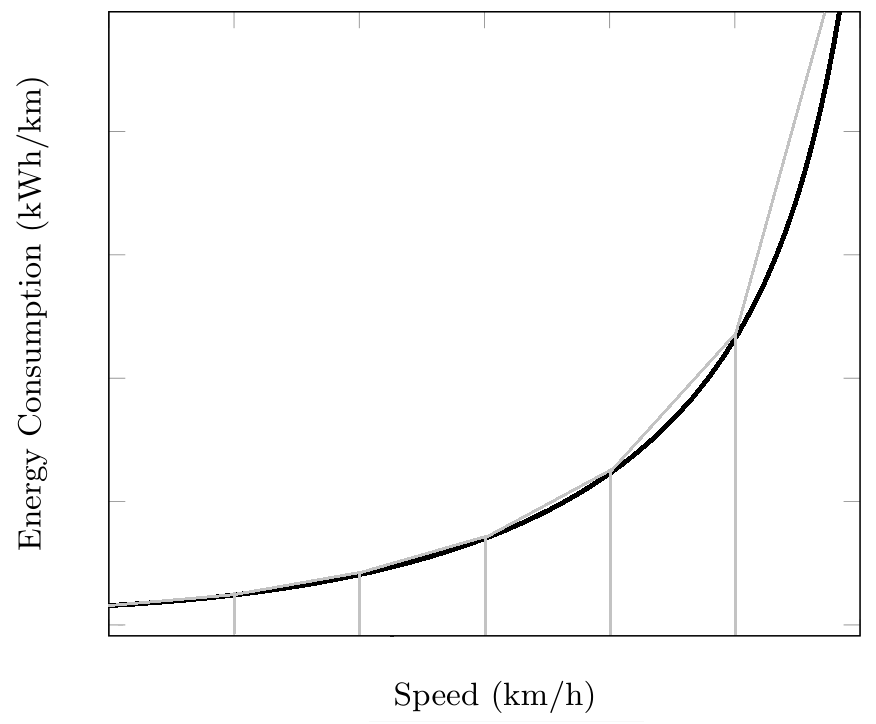
\includegraphics[scale=0.33]{images/linearization_example}
\label{fig:linearization_example}
\end{center}

$n$ is the length of the path, $m$ is the amount of lines the functions \( D(e_i)/v_{e_i} \) and $R_{CO}(v_{e_i})$ are split into and $\sum_{j=1}^{m} SL_{i,j} = 1$ ensures that only one line segments can be selected.
Being that exactly one line segment needs to be chosen. In other words, SL needs to be binary values.
\begin{equation*}
\forall_{i\in1 \dots n, j \in 1 \dots m}: \; \; SL_{i,j} \in{0,1} 
\end{equation*}
The speed of the EV needs to be constrained by the line segment chosen:
\begin{equation*}
\forall_{i\in1 \dots n, j \in 1 \dots m-1}:\; SL_{i,j} * P_{i,j}  \le  v_{j,e_i} \le SL_{i,j}*P_{i,j+1}
\end{equation*}

$P$ is a set of starting points of all line segments including the end point of the last segment. $SL_{i,j} * P_{i,j}$ is the minimal speed the EV is allowed to drive on edge $i$ and $SL_{i,j}*P_{i,j+1}$ is the maximal speed, note that the values will either be a valid value or $0$ if the segment is not selected. $P_{i,j+1}$ is the end point of $P_{i,j}$. 
The approximate solution to \( D(e_i)/v_{e_i} \) or $R_{CO}(v_{e_i})$ can now be found by precomputing the functions of each of the individual linear lines \( D(e_i)/v_{e_i} \) or $R_{CO}(v_{e_i})$ is split into, the produce precomputing is a set of slopes called $LinesA$ and a set constants called  the  multiplying the slope of the selected line with the selected speed and adding the constants called $LinesB$. As an example the way to model $R_{CO}(v_{e_i})$ for $i$
\begin{equation*}
\sum_{j=1}^{m} LinesA_{i,j}*v_{j,e_i} + \sum_{j=1}^{m} SL_{i,j}*LinesB_{i,j} 
\end{equation*}
$\sum_{j=1}^{m} LinesA_{i,j}*v_{j,e_i}$ is equlent of $a*x$ and $\sum_{j=1}^{m} SL_{i,j}*LinesB_{i,j}$ is equivalent with $b$ and thus the consumption rate of the EV is modeled as $m$ function in linear form $a*x + b$. 
Finally note that this is a way to determine the solution of \( D(e_i)/v_{e_i} \) or $R_{CO}(v_{e_i})$ and before the solution can be found the line segments and points for each of both of the non linear functions needs to be precomputed. 
%sources
%1, SWP-3587
%2, glpk-sos2


